\chapter{Results}
\label{chap:results}

When developing a new algorithm, an important part is testing and evaluation
against existing solutions. This chapter describes this stage, informing about a data set used to debug and improve our solution, and the method of comparison with other solutions, such as fermikit and GATK. The last part of the chapter covers certain variants that proved to be interesting when examined by our algorithm.

\section{Test Data Set}
\label{sec:test-data-set}

 chr1:1-40,000,000 region of the high-coverage
data from the 1000 Genome Project. In addition to the input reads \cite{testreads}, also variants called by fermikit and GATK are available in form of VCF files \cite{testvcf}. The VCF files were used to compare the accuracy of the algorithm. In order to be able to make meaningful comparisons and to avoid remapping of all reads, we used the same version of the reference genome which was used also by the 1000 Genome Project (GRCh37 \cite{testref}).

The test read set consists of 12,475,011 reads with lengh of 151 bases. Figure \ref{fig:test-kmer-frequency-distribution} shows k-mer frequency distribution of the set with k-mer size of 21 bases. The shape of the graph, when compared to Figure \ref{fig:kmer-frequency-distribution} suggests that the set indeed contains read errors, therefore the error correction step was applied.

\begin{figure}[h]
\centering
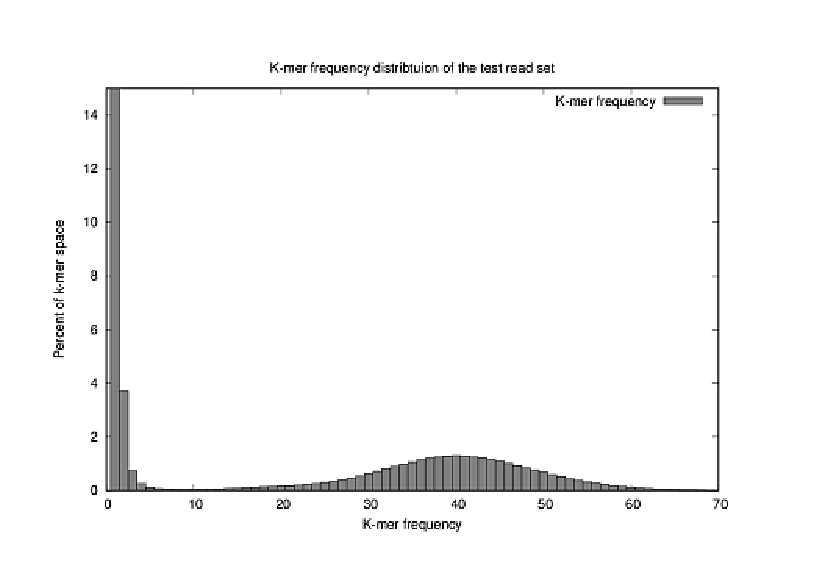
\includegraphics{img/test-kmer-frequency-distribution.pdf}
\caption{K-mer frequency distrubtion of the raw input read set}
\label{fig:test-kmer-frequency-distribution}
\end{figure}

As Table \ref{tab:test-correction} indicates, the error correction process removed and shortened a signifficant proportion of the reads. Approximately 21\% of the input reads was subject to repairs. Figure \ref{fig:test-repair-frequency} shows a distribution of the number of repaired bases per read, not including effects of read trimming.

\begin{table}[h]
\begin{center}
\caption{Statistics related to error correction of the test data set}
\label{tab:test-correction}
\begin{tabular}{| c | c | p{5cm} |}
\hline
Category & Value & Percentage \\
\hline
Total reads & 12,475,011 & - \\
\hline
Removed & 64,653 &  $0.52$\% of all reads. \\
\hline
Shortened & 944 & $0.0076$\% of all reads \\
\hline
Total bases & 1,880,123,991 & - \\
\hline
Bases repaired & 5,098,764 &  $0.27$\% of all bases \\
\hline
\end{tabular}
\end{center}
\end{table}

\begin{figure}[h]
	\centering
	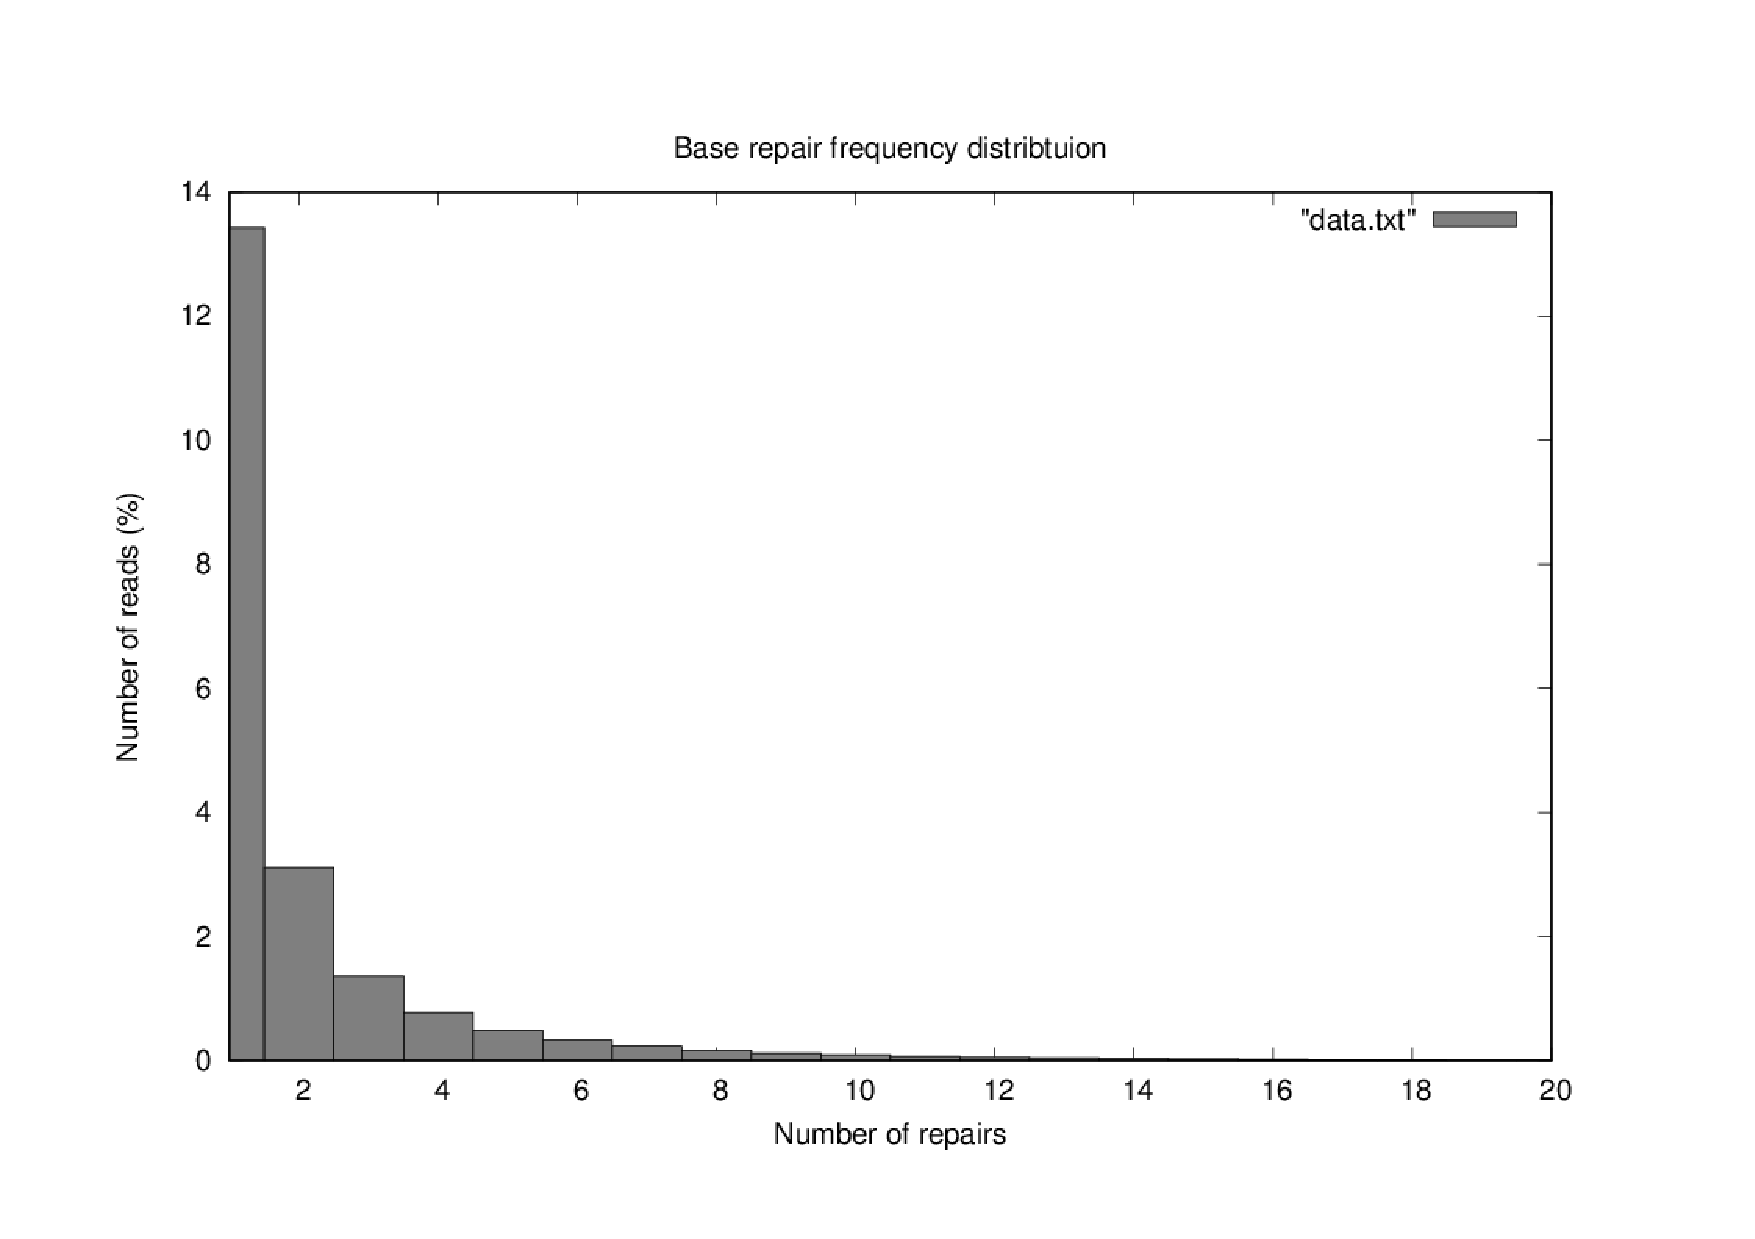
\includegraphics{img/test-repair-frequency.pdf}
	\caption{Distribution of a number of repaired bases in a single read}
	\label{fig:test-repair-frequency}
\end{figure}

Figure \ref{fig:test-kmer-frequency-distribution2} shows the k-mer frequency distribution of the corrected read set. Although still not perfect, the distribution of corrected reads resembles the theoretical distribution of an ideal error-free set more than the distribution of raw reads.

\begin{figure}[h]
\centering
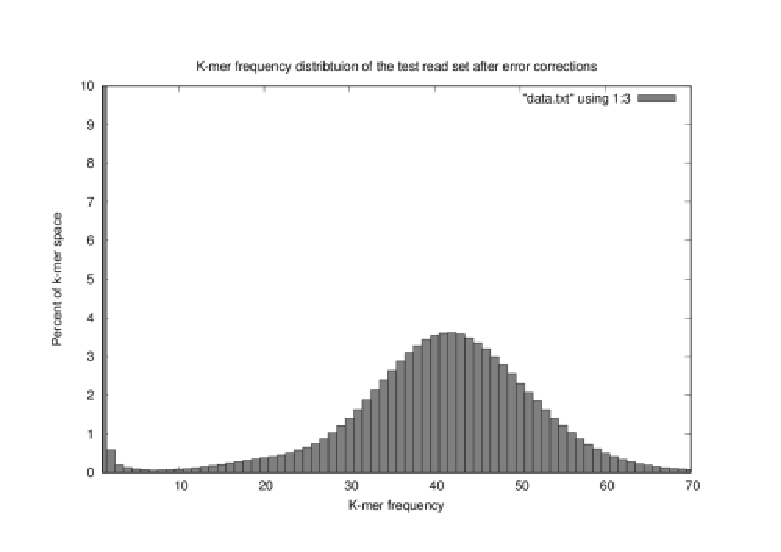
\includegraphics{img/test-kmer-frequency-distribution2.pdf}
\caption{K-mer frequency distrubtion of the corrected read set}
\label{fig:test-kmer-frequency-distribution2}
\end{figure}

As described in Section \ref{sec:input-output-and-preprocessing}, not all input reads, even from the corrected set, can be processed by our algorithm. Table \ref{tab:corrected-set-categories} summarizes numbers of reads discarded for various reasons. The preprocessing phase removed nearly one fifth of the corrected data set (18.99\%). Most of the reads were removed due to being possible duplicates (87.65\%). Quite a large portion of  reads were not accepted because of their low mapping quality (12.97\%). Also, about 3\% of all the reads were shortened in order to remove soft-clipped regions.

\begin{table}[h]
\begin{center}
\caption{Categories of reads present within the corrected test data set}
\label{tab:corrected-set-categories}
\begin{tabular}{| c | c | p{5cm} |}
\hline
Name & Value & Percentage \\
\hline
Total reads & 12,410,475 & - \\
\hline
Bad reads & 2,357,002  & $18.99$\% of all reads \\
\hline
Low MAPQ & 305,588 & $12.97$\% of bad reads \\
\hline
Unmapped & 5,020 & $0.21$\% of bad reads \\
\hline
Supplementary & 33,621 & $1.43$\% of bad reads \\
\hline
Duplicate & 2,065,795 & $87.65$\% of bad reads \\
\hline
Soft-clipped & 305,209 & $3.04$\% of accempted reads \\
\hline
\end{tabular}
\end{center}
\end{table}

\section{Quality Evaluation}
\label{sec:quality-evaulation}

In order to evaluate the algorithm, the generated VCF files were compared to those generated by the following variant calling toolchains:
\begin{itemize}
\item \textbf{GATK}. These VCFs were taken as reference points, since the method used by GATK should be very similar to our algorithm. Hence, results of all algorithms were compared against them.
\item \textbf{Fermikit}. Unlike GATK and our algorithm, Fermikit's assembly algorithm is based on the OLC concept.
\item \textbf{Fermikit on regions}. This is a combination of the OLC approach used by Fermikit and the short region one adopted by our algorithm (and also by GATK). The fermikit assembly algorithm was run on exactly the same regions as our algorithm. The aim of this test case was to force the Fermikit to minimize differences of outputs generated by DBG and OLC algorithms.
\item \textbf{samtools mpileup, bcftools call}. A traditional variant caller implemented by SAMtools and BCFtools packages \cite{samtools}.
\end{itemize}

Results generated by these algorithms were compared to those of GATK using the tool\textbf{ rtgeval}. Rtleval is a wrapper for RTG's vcfeval, a sophisticated open source variant comparison tool developed by Realtime Genomics. It simplifies the use of vcfeval and potentially helps to get consistent results given VCFs produced by different variant callers \cite{rtgeval}.

Rtgeval accepts two VCF files on input: a test set and a truth set. The truth set is a VCF file generated by a reference algorithm, in our case GATK. The test set VCF is produced by the algorithm to be tested. The evaluation is done separately for SNPs and indels and each variant is sorted into one of three categories:
\begin{itemize}
\item \textbf{True positive (TP)}. The variant is present in both sets.
\item \textbf{False negative (FN)}. It is present in the truth set only.
\item \textbf{False positive (FP)}. It can be found only in the test set.
\end{itemize}

Rtgeval can compare VCF files in three different modes: positional, allelic and genotypic. The positional mode is intuitive; the tool is determining whether the same varaints are present at approximately the same position inside both test and truth set. If the positions difference does not exceed 10 bases, the variants are considered true positives. Otherwise, either false negative, or fale positive is reported. In allelic mode, the tool focuses on biallelic variants and evaluates whether they are correctly detected by both tested algorithms. The genotyping mode compares genotype and phasing information of the variants.

\subsection{Positional}
\label{subsec:positional-results}

The comparison in positional mode is shown in Table \ref{tab:positional-results}. It is clear that variants called by OLC and DBG classes of algorithms indeed are not the same. The percentages were counted from the total number of variants in GATK's VCF file, separately for SNPs and indels.

Fermikit, as a representative of the OLC class, performs well when looking at numbers of false positives (below 1\% in case of SNPs, \textasciitilde 2.3\% indels), which is, however, trated off by quite  big percentage of undetected variants (about 10\% for SNPs and 28\% indels). Numbers of false negatives are reduced when the algorithm is run on the region basis, although false positives roughly triple. Such situation seems to be typical also for other algorithms or different parameter settings of one algorithm; when the number of false negatives drops, false positives rise and vice versa.

Our algorithm was run with default settings described in Section \ref{sec:algorithm-parameters}. The value of 4 for the global threshold is, compared for example to HaploCall that uses 2, high. It was chosen to fight high numbers of false positives. The default settings actually removes the binomial test from the variant filtering process since no low quality variants actually emerge. As discussed later, the binomial test, although useful in some cases, did not prove to be a world-saver.

When talking about SNPs, results produced by the SAMTools and BCFTools tandem form quite the opposite to those of the Fermikit run at the whole genome. Less than 3\% of SNPs found by GATK were left undiscovered, however, howerver, the number of false positives increased. It is true that our algorithm did not achieved nearly the same number of false negatives even when run with low global threshold causing loads of false positives.

\begin{table}
\begin{center}
\caption{Positional comparison of results generated by our algorithm}
\label{tab:positional-results}
\begin{tabular}{| c | c | c | c | p{3cm} |}
\hline
/ & Fermikit & Fermikit (regions) & mpileup & Our algorithm \\
\hline
SNP TP & 45,241 (89.3\%) & 47,650 (94\%) & 49,201 (97.1\%) & 48,117 (94.96\%) \\
\hline
SNP FN & 5,432 (10.7\%) & 3,043 (6\%) & 1,472 (2.9\%) & 2,556 (5.04\%) \\
\hline
SNP FP & 385 (0.76\%) & 1,441 (2.84\%) & 2,090 (4.12\%) & 803 (1.58\%) \\
\hline
INDEL TP & 7,853 (71.6\%) & 9,802 (89.4\%) & 8,707 (79.39\%) & 9,468 (86.43\%) \\
\hline
INDEL FN & 3,114 (28.4\%) & 1,365 (10.6\%) & 2,260 (20.61\%) & 1,499 (13.57\%) \\
\hline
INDEL FP & 250 (2.28\%) & 835 (7.61\%) & 1,412 (12.95\%) & 1,242 (11.32\%) \\
\hline
\end{tabular}
\end{center}
\end{table}

A deeper analysis of the results obtained by running our algorithm with lower values of the global threshold (2 and 3 to be precise) and different initial k-mer sizes suggests that the variant filtering step needs additional work to be done. It is true that information stored inside the variant graph can be used to get hints what variants should be filtered out. Variants with the reference and alternate sequences covered by the same reads, or paired-end reads seem to be, at first glance, good candidates for false positives. Unforunately, these information need not to be treated as hard facts. Simply classifying variants with such properties ad false positives did not bring expected results. Furthermore, coloring restrictions of the variant graph do not permit to deduce genotypes for such cases.

Also, the analysis suggested that many of the undetected GATK variants were removed because of their low read coverage. Low number of supporting reads was not, howerver, cuased by a sequencing error, but by a lower read coverage of the whole active region. Hence, introducing a binomial test to resolve such cases seemed to be a good idea. Effects of the test addition were observed more closely on our algorithm run with the initial k-mer size set to 31, and global threshold to 2. Figure \ref{fig:binom-all} shows number of TPs and FPs filtered out when the binomial test was applied to all called variants. Figure \ref{fig:binom-3} is a result of applying the test only to variants with less than 4 supporting reads (the low quality variant threshold set to 3).

\begin{figure}
	\centering
	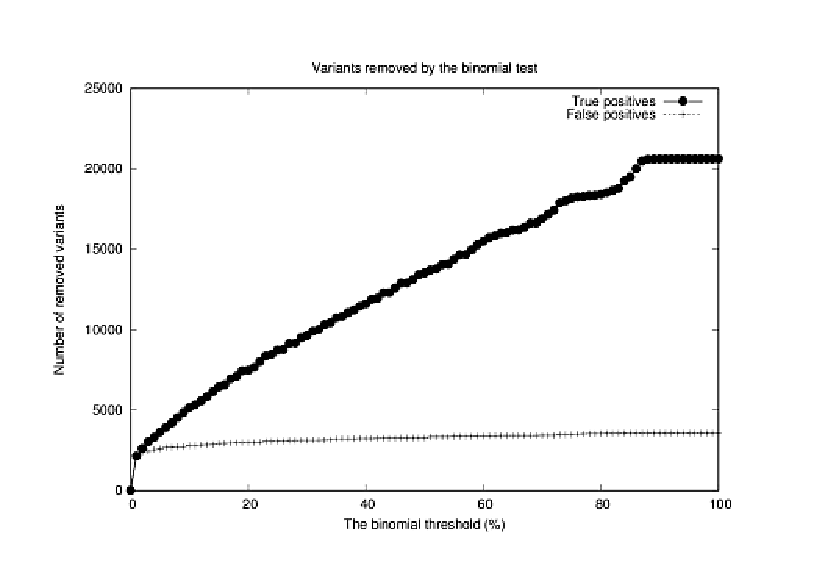
\includegraphics{img/binom-all.pdf}
	\caption{Numbers of TPs and FPS removed by the binomial test applied to all called variants}
	\label{fig:binom-all}
\end{figure}

\begin{figure}
	\centering
	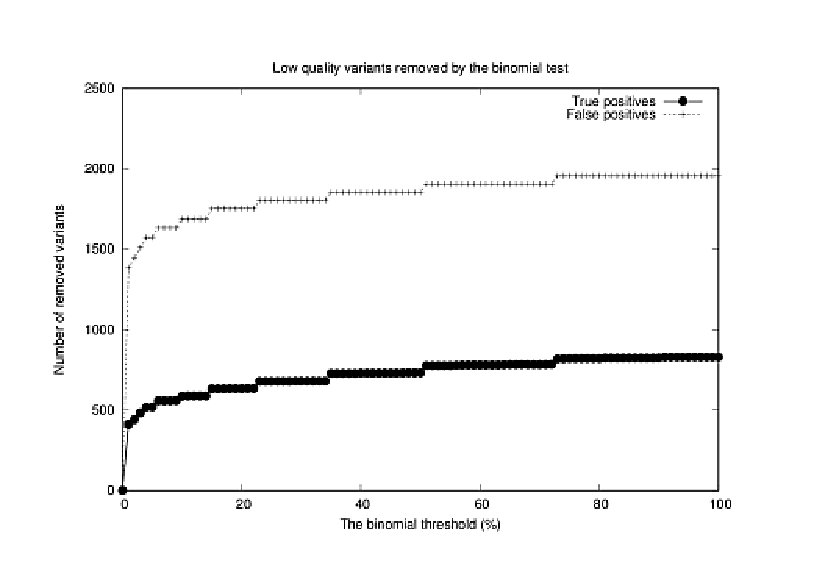
\includegraphics{img/binom-3.pdf}
	\caption{Numbers of TPs and FPS removed by the binomial test applied to variants with less than 4 supporting reads}
	\label{fig:binom-3}
\end{figure}

The test run produced a total of X variants shared with GATK's VCF, and Y false positives. As Figure \ref{fig:binom-all} illustrates, even setting value of the binomial threshold to 1\% removed about 6000 of true positives. Although this is roughly only 10\%, we do not consider the case as a good trade-off even with regard to percentage of removed false positives (50\%). 

When applied only to the variants with low read support, the binomial test gives much more sense. Setting the binomial threshold to 1\% removes only X true positives but has great effect on sorting out the false variants. Unfortunately, we do not consider the effect as great enough, since running our algorithm with lower global threshold produces more false positives than the binomial test removes.
